
\documentclass{article}
\usepackage{graphicx}
\usepackage{mathpazo}
\pagestyle{empty}

\begin{document}
  \begin{picture} (200.000000,200.000000)(0,0)
    \put(0.0, 0.0){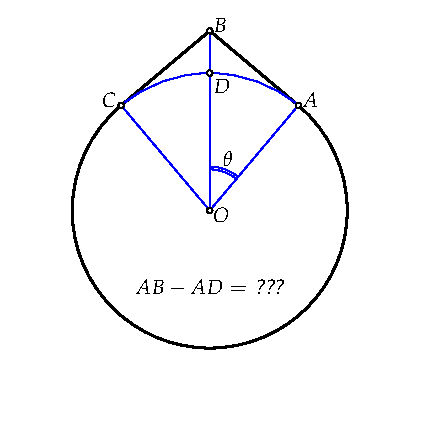
\includegraphics{02string-around-earth.eps}}
    \put(102.00,  95.00){\sffamily\itshape \makebox[0pt][l]{$O$}}
    \put(144.52, 150.48){\sffamily\itshape \makebox[0pt][l]{$A$}}
    \put(102.00, 186.29){\sffamily\itshape \makebox[0pt][l]{$B$}}
    \put( 55.48, 150.48){\sffamily\itshape \makebox[0pt][r]{$C$}}
    \put(102.00, 157.00){\sffamily\itshape \makebox[0pt][l]{$D$}}
    \put(106.60, 121.78){\sffamily\itshape \makebox[0pt][l]{$\theta$}}
    \put(100.00,  60.40){\sffamily\itshape \makebox[0pt][c]{$AB-AD = $ ???}}

  \end{picture}
\end{document}

